%%% Local Variables:
%%% mode: latex
%%% TeX-master: "cheat-sheet"
%%% End:

When a process blocks, it does so because logically it cannot continue, typically because it is waiting for input that is not yet available.

It is also possible for a process that is conceptually ready and able to run to be stopped because the operating system has decided to allocate the CPU to another process for a while.

These two conditions are \emph{completely different}. In the first case, the suspension is inherent in the problem (you cannot process the user' s command line until it has been typed). In the second case, it is a technicality of the system (not enough CPUs to give each process its own private processor).

The three possible states:
\begin{description}
\item[Running] Actually using the CPU at that instant
\item[Ready] Runnable; temporarily stopped to let another process run
\item[Blocked] Unable to run until some external event happens
\end{description}

\begin{figure}[H]
  \centering
  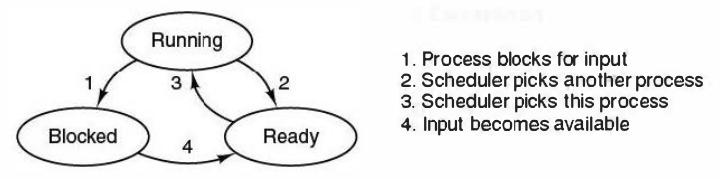
\includegraphics[scale=0.5]{images/thread_life}
  \caption{Transition diagram of thread states}
\end{figure}
